% Template LaTeX source file for homework problem solutions.
% Alan T. Sherman (9/9/98)

% Running LaTeX
%
% Name this file FOO.tex
% latex FOO
% latex FOO   
%    (You have to run latex twice to get the cross references correct.
%     Running latex creates a file FOO.dvi 
%     You can view dvi files with the program xdvi )
% xdvi FOO.dvi &
%
% lpr -d FOO.dvi
%    (To print the dvi file.   Be sure to use the "-d" print option,
%     and be sure your printer can handle dvi files (not all printers can).
%     Do NOT print with "lpr FOO.dvi", which will print tens of pages
%     of unreadable dvi source code. Printing a postscript (ps) file
%     is usually more reliable, as explained below.)
%
% dvips FOO.dvi
%    (To create a postscript file named FOO.ps 
%     which you can view with the program ghostview )
% ghostview FOO.ps &
% lpr FOO.ps
%    (To print the ps file.)

%%%%%%%%%%%%%%%%%%%%%%%%%%%%%%%%%%%%%%%%%%%%%%%%%%%%%%%%%%%%%%%%%%%%%%

\documentclass[12pt]{article}
\usepackage{amsmath,amssymb}
\usepackage{graphicx}

% Set the margins
%
\setlength{\textheight}{8.5in}
\setlength{\headheight}{.25in}
\setlength{\headsep}{.25in}
\setlength{\topmargin}{0in}
\setlength{\textwidth}{6.5in}
\setlength{\oddsidemargin}{0in}
\setlength{\evensidemargin}{0in}




%%%%%%%%%%%%%%%%%%%%%%%%%%%%%%%%%%%%%%%%%%%%%%%%%%%%%%%%%%%%%%%%%%%%%%%
% Macros

% Math Macros.  It would be better to use the AMS LaTeX package,
% including the Bbb fonts, but I'm showing how to get by with the most
% primitive version of LaTeX.  I follow the naming convention to begin
% user-defined macro and variable names with the prefix "my" to make it
% easier to distiguish user-defined macros from LaTeX commands.
%
\newcommand{\myN}{\hbox{N\hspace*{-.9em}I\hspace*{.4em}}}
\newcommand{\myZ}{\hbox{Z}^+}
\newcommand{\myR}{\hbox{R}}

\newcommand{\myfunction}[3]
{${#1} : {#2} \rightarrow {#3}$ }

\newcommand{\myzrfunction}[1]
{\myfunction{#1}{{\myZ}}{{\myR}}}


% Formating Macros
%

\newcommand{\myheader}[4]
{\vspace*{-0.5in}
\noindent
{#1} \hfill {#3}

\noindent
{#2} \hfill {#4}

\noindent
\rule[8pt]{\textwidth}{1pt}

\vspace{1ex} 
}  % end \myheader 

\newcommand{\myalgsheader}[0]
{\myheader{METU, Computer Engineering}
{CENG564 - Pattern Recognition THE "2" \\ "{\bf Deniz Uluğ}"  - "2172088" "{\bf Kaan Hamilton}"  - "2035962"} {Fall 2016}{}}

% Running head (goes at top of each page, beginning with page 2.
% Must precede by \pagestyle{myheadings}.
\newcommand{\myrunninghead}[2]
{\markright{{\it {#1}, {#2}}}}




%%%%%% Begin document with header and title %%%%%%%%%%%%%%%%%%%%%%%%%

\begin{document}

\myalgsheader
\pagenumbering{gobble}
\pagestyle{plain}



\section*{Questions} 

% fill the blanks with your answers
\section*{Answer 1}
% answer of question 1 goes here etc..

Let $\bar{X} = \{3,5,7\}$, $\bar{Z} = \{0,1\}$, $\bar{Y} = \{10,20,30\}$. Where the sets are the possible values of the respective random variables. We assume that all other probabilities of other values for each random variable is zero. This is correct since respective columns and rows add up to 1 at each case.\\

i. $P(Z=1 | X=7) =  \dfrac{(Z=1, X=7)}{P(X=7)} = \dfrac{0.21}{0.30}=0.7$ \\ Where $P(X=7) = \sum_{i\in \bar{Y},j\in \bar{Z}  } P(X=7,Y=i,Z=j)$ which we can infer each term directly from the table.\\

ii. 
\[ P(X=x) = \begin{cases} 
      0.3 & x = 3 \\
      0.4 & x=5 \\
      0.3 & x=7 \\
      0 & otherwise 
   \end{cases}
\] \\

    Where for all $n \in \bar{X}$, we can infer $P(X=n) = \sum_{i\in \bar{Y},j\in \bar{Z}  } P(X=n,Y=i,Z=j)$ where we know the each joint probability term by the given table.\\
    
        iii. 
    $E_x[X] = \sum_{i\in\bar{X}} P(i)i = 3 \cdot \dfrac{3}{10}+ 5\cdot \dfrac{4}{10}+ 7\cdot \dfrac{3}{10} = 5 $ \\
    
    Let us denote this expected value as $\mu_x$ \\
    
    $Var_x[X] = E_x[ (X - \mu_x)^2 ] = \sum_{i\in\bar{X}} P( i )(i-\mu_x)^2 = 0.3\cdot 4 + 0.4\cdot 0 + 0.3 \cdot 4 = 2.4$ \\
    
%    Where it can be shown that the term $P( (i-\mu^2) )$ is equal to just $P(i)$
    iv.
	For all $n\in \bar{X}$,	$P( X = n | Z=1) = \dfrac{P(X=n, Z=1)  }{P(Z=1)}$ \\
	
	For the denominator, $P(Z=1) = \sum_{i\in \bar{Y},j\in \bar{X}  } P(X=j,Y=i,Z=1)= 0.685$ , where we can infer each term directly from the table. \\
	
	For numerator, $P(X=n, Z=1) =  \sum_{i\in \bar{Y}} P(X=n,Y=i,Z=1)$ where again we can infer each term directly from the table. \\
	
	Putting all together and rounding up to 4 significant value; 
	\[ P(X =x | Z = 1 ) = \begin{cases} 
       0.2847 & x = 3 \\
      0.4088 & x=5 \\
      0.3066 & x=7 \\
      0 & otherwise 
   \end{cases}
\] \\

       v.
    $E_{X|Z=1}[x] = \sum_{i\in\bar{X}} P(i|Z=1)i = 3 \cdot 0.2847+ 5\cdot 0.4088+ 7\cdot 0.3066 = 5.0438 $ \\
    
    Let us denote this expected value as $\mu_{x2}$ \\
    
    $Var_x[X] = E_x[ (X - \mu_{x2})^2 ] = \sum_{i\in\bar{X}} P( i )(i-\mu_{x2})^2 = 0.2847\cdot 4.1771 + 0.4088\cdot 0.0019 + 0.3066 \cdot 3.8267 = 2.3630$ \\
    
\section*{Answer 2}

Assuming $X$ is choosen uniform randomly;

i. By the pdf of the uniform distribution:

	\[ f( x ) = \begin{cases} 
       \dfrac{1}{90} & x \in [10,100] \\
      0 & otherwise 
   \end{cases}
\] \\
% \displaystyle\int\limits_a^b  
And $P(I=[a,b]) = P(a\leq x \leq b) = \displaystyle\int\limits_a^b  f(x)dx = \displaystyle\int\limits_a^b   \dfrac{1}{90} = \dfrac{b-a}{90} $ \\

ii. $E_X[x] = \displaystyle\int\limits_{10}^{100} xf(x)dx =  \displaystyle\int\limits_{10}^{100}  \dfrac{x}{90}dx =\frac{500}{9}-\frac{5}{9} = 55   $ \\

iii. It is easy to show that the roots of the equation are $40$ and $70$, and the equation is positive between $[10,40)$ and $(70,100]$ and negative in $(40,70)$. Given that, the probabilty of the equation being positive is: \\

$P(X^2-110X+2800>0) = 1 - P(40 \leq x \leq 70) = 1 -  \dfrac{70-40}{90} = 0.6666 $ by part i. \\

Also note that since the probability of "single points" are zero for continous distributions, like this one, $\leq$ and $<$ makes no difference above. \\

iv. The integral of the density function should equal zero. Therefore: \\

$  \displaystyle\int\limits_{-\infty}^{+\infty} f(x)dx  = \displaystyle\int\limits_{10}^{100} f(x)dx = \displaystyle\int\limits_{10}^{100}Cxdx =C ( \frac{100^2}{2}-\frac{10^2}{2}) = C\cdot 4950 = 1$ \\ 

Therefore, $C=\dfrac{1}{4950} $ and $f(x) = \d1frac{x}{4950} $ \\

And $E_X[x] = \displaystyle\int\limits_{10}^{100} xf(x)dx =  \displaystyle\int\limits_{10}^{100}  \dfrac{x^2}{4950}dx =\frac{20000}{297}-\frac{20}{297} = \frac{740}{11} $ \\



\section*{Answer 3} 

\quad i. Let $Y=\sqrt{|X|} $ be a random variable (as it already is). We can start by considering cdf of $Y$. Let $F_X(x)$ be the cdf of $X$ and $F_Y(x)$ of Y. It is easy to see that $Y$ is always positive, and $Y$ is "bounded" by the probabilty of $X$ which means $f_Y(x)=0$ for $x\notin [-1,1]$. So assume $x\in [0,1]$: \\

$F_Y(x) = P(Y<x) = P( \sqrt{|X|} < x) = P( |X| < x^2 ) = P( -x^2 < X < x^2 ) = $ \\ 

$P( X < x^2) - P( X < -x^2 ) = F_X(x^2) - F_X(-x^2) $ \\ 


The third equality is possible because square root is a monotonically increasing function. Taking derivative of both sides: \\

$f_Y(x) =2xf_X(x^2)+2xf_X(-x^2)$ \\

Note that when $x\in [-1,1]$, so does $x^2$ and $-x^2$ too. Then since we know $f_X$ by the definition of pdf of uniform random variable:\\

$f_Y(x) = 2x(\dfrac{1}{2}+\dfrac{1}{2})=2x $

\[ f_Y( x ) = \begin{cases} 
		2x & 0 < x < 1        \\
       0 & otherwise
      
   \end{cases}
\] \\


ii. Let $Z= -ln|X|  $ be a random variable (as it still already is). We can still start by considering cdf of $Z$. Let $F_X(x)$ be the cdf of $X$ and $F_Z(x)$ of Z.\\

$F_Z(x) = P(Z<x) = P( -ln|X| < x) = P( ln|X| > -x) =P( |X| > e^{-x} ) =$\\

$ 1 - P( |X| < e^{-x} ) = 1 - P( e^{-x} < X < e^{-x} ) = 1- P( X < e^{-x} ) + P( X < -e^{-x} ) = $\\

$1-F_X(e^{-x}) + F_X(-e^{-x})$\\


The fourth equality is possible because $ln$ is a monotonically increasing function. Taking derivative of both sides: \\

$f_Z(x) =e^{-x}f_X(e^{-x})+ e^{-x} f_X(-e^{-x})$ \\

Notice that when $e^{-x}\in [-1,1]$, $x\in [0,\infty)$. When $-e^{-x}\in [-1,1]$, $x\in [0,\infty)$. So take $x$ in that region:\\

$f_Z(x) =e^{-x}  (\dfrac{1}{2}+\dfrac{1}{2}) =e^{-x} $

\[ f_Z( x ) = \begin{cases} 
		e^{-x} & 0 < x \\
       0 & otherwise
      
   \end{cases}
\] \\

Also note that, again since the random variables are contionus, $\leq$ and $<$ makes no difference.




\section*{Answer 4}

Assuming the coordinates are on the edges of the triangle, this implies $X \sim U(0,1)$ and $Y \sim U(-1,1)$. \\

Take $Z=X-Y$ (we will include absolute operator later). \\

$F_Z(z) = P(Z<z) = \displaystyle\int\limits_{-\infty}^{+\infty} P(Z<z|X=x)dF_X(x)  $\\

$ = \displaystyle\int\limits_{-\infty}^{+\infty} P(X-Y<z | X=x)dF_X(x) $ \\

Notice that since it is given $X=x$, $X=x$.\\

$ = \displaystyle\int\limits_{-\infty}^{+\infty} P(x-Y<z | X=x)dF_X(x) $ \\

$ = \displaystyle\int\limits_{-\infty}^{+\infty} P( x-z <Y )dF_X(x) $ \\

$ = \displaystyle\int\limits_{-\infty}^{+\infty} ( 1-  F_Y(x-z) )  dF_X(x) $ \\

Now, what we have here is a Riemann-Stieltjes integral. Since by definition $F_X$ is differentiable, we can write:

$ = \displaystyle\int\limits_{-\infty}^{+\infty} ( 1-  F_Y(x-z) ) f_X(x)dx $ \\ 

Now it is given that $X$ is a uniform distribution, and since it is on the given triangle its range is $[0,1]$. Let's break our integral in to three pieces, as $f_X(x) = 1$ when $x\in [0,1]$ and $0$ otherwise:

$ =\displaystyle\int\limits_{-\infty}^{0} ( 1- F_Y(x-z) ) f_X(x) dx + \displaystyle\int\limits_{0}^{1} ( 1- F_Y(x-z) ) f_X(x) dx $\\$+ \displaystyle\int\limits_{1}^{+\infty} ( 1- F_Y(x-z) ) f_X(x) dx $ \\ 

$ =\displaystyle\int\limits_{-\infty}^{0} ( 1- F_Y(x-z) ) 0dx + \displaystyle\int\limits_{0}^{1} ( 1- F_Y(x-z) ) 1dx + \displaystyle\int\limits_{1}^{+\infty} ( 1- F_Y(x-z) ) 0dx $ \\ 

$ = \displaystyle\int\limits_{0}^{1} ( 1- F_Y(x-z) ) dx  $  \\

Let's open $F_Y$ for better inspection:

\[  F_Y(x-z)  = \begin{cases} 
		0 & x < z-1 \\
		\dfrac{x-z+1}{2} &  z-1 \leq x < 1 + z \\
		1 & 1+z \leq x
      
   \end{cases}
\] \\

Remember that $x$ varies between $[0,1]$ and $z$ is fixed since the beginning.  So there are three cases to consider. (1) If $z>2$, $F_Y(x-z)$ evaluates to $0$ for all such $x$ and integral itself evaluates to $1$, (2) if $z<-1$, $F_Y(x-z)$ evaluates to $1$ for all such $x$ and integral itself evaluates to $0$, (3) if $z\in [-1,2]$:\\

In third case we again need to consider three cases, (1) $z-1\in [0,1]$ so $z\in [1,2]$, (2) $z+1\in [0,1]$ so $z\in [-1,0]$ and (3) $z\in [0,1]$ so $[z-1,z+1] \supset [0,1]$. Let's evaluate our integral for each case one by one. \\

(1) $F_Z(z) =  \displaystyle\int\limits_{0}^{z-1} (1-0)dx + \displaystyle\int\limits_{z-1}^{1} (1-\dfrac{x-z+1}{2}) dx $ \\ 

$ = z-1 +\dfrac{-z^2+4}{4}$ \\

(2) $F_Z(z) =  \displaystyle\int\limits_{0}^{z+1} (1-\dfrac{x-z+1}{2})  dx + \displaystyle\int\limits_{z+1}^{1} (1-1) dx $ \\ 

$ = \dfrac{z^2+2z+1}{4} +0$ \\

(3)$ F_Z(z) = \displaystyle\int\limits_{0}^{1} (1-\dfrac{x-z+1}{2}) dx $ \\ 

$ = \dfrac{z+1}{2}-\dfrac{1}{4} $ \\ 

So:

\[  F_Z(z) = \begin{cases} 
		0 & z < -1\\
        \dfrac{z^2+2z+1}{4} & -1 < z < 0 \\
       \dfrac{z+1}{2}-\dfrac{1}{4}  & 0 < z < 1 \\ 
        z-1 +\dfrac{-z^2+4}{4} & 1 < z < 2 \\
       1 & 2 < z \\
      
   \end{cases}
\] \\

\[  f_Z(z) = \begin{cases} 
		0 & z < -1\\
     	\dfrac{z+1}{2}   & -1 < z < 0 \\
       \dfrac{1}{2}& 0 < z < 1 \\ 
        \dfrac{2-z}{2} & 1 < z < 2 \\
       0 & 2 < z \\
      
   \end{cases}
\] \\

Now finally define random variable $T = |Z| = |X-Y|$ \\

$F_T(t) = P(T<t) = P(|Z|<t) = P( -t < Z < t) = F_Z(t) - F_Z(-t) $ \\

Taking derivatives of both side: \\

$f_T(t) = f_Z(t)+f_Z(-t) $\\


\[  f_T(t) = \begin{cases} 
		0 & z < -2		\\
		\dfrac{2-z}{2} & -2 < z < -1\\
     	\dfrac{z+2}{2} & -1 < z < 0 \\
       \dfrac{z+2}{2} & 0 < z < 1 \\ 
       \dfrac{2-z}{2} & 1 < z < 2 \\
       0 & 2 < z \\
      
   \end{cases}
\] \\

\section*{Answer 5}
\quad Let $E(X)=\mu_X$. Also note that expectancy satisfies the following property, where $c$ is a constant and $u$ is a function: \\

$E(c_1\cdot u_1(X) + c_2\cdot u_2(X)  ) = c_1\cdot E(u_1(X)) + c_2\cdot E( u_2(X) ) $ \\

i. By definition, we know that the right hand side equals variance: \\

$E[ (X-\mu_X)^2 ] = Var(X) = \sigma^2_X $ \\

Now let's look at $E(X^2)$:

$E(X^2) = E[ (X-\mu_X+\mu_X)^2 ] =  E[  (X-\mu_X)^2 + 2(X-\mu_X)\mu_X + \mu_X^2  ]$ \\

$= E[(X-\mu_X)^2] + 2E(X-\mu_X) + E(\mu_X^2) $\\

$ = \sigma_X^2 + 2E(X) - 2E(\mu_X) + E(\mu_X^2) $ \\

$ = \sigma_X^2 +2\mu_X -2\mu_X + \mu_X^2 = \sigma_X^2 + \mu_X^2 $ \\

Let's put all together, the left hand side is equal to:\\

$E(X^2)-E(X)^2 = \sigma_X^2 + \mu_X^2 - \mu_X^2 = \sigma_X^2 = E[ (X-\mu_X)^2 ]  $ \\

Which is just what we had said right hand side to be. \\

ii. Let $h(Y) = E_{X|Y}(X|Y) = \sum_x xP(x|Y) $, which is a random variable itself depending on the random variable $Y$. Note that the second equality is by definition of conditional expectance. Then the right hand side is:\\

$E_Y( E_{X|Y}(X|Y)  )  = E_Y(h(Y)) = \sum_y h(y)P(y) =  $\\

$ \sum_y \sum_x xP(x|y)  P(y)    = \sum_y \sum_x xP(x,y)   =\sum_x xP(x) = E(X)  $ \\

Which is just the left hand side. \\

iii. It is given that $Var(X) = Var(Y) = \sigma^2 $. Denote $Z=X-Y$ and $T=X+Y$. We wish to show $cov(Z,T)=0$.  First note that: \\

$\mu_T = E(T) = E(X+Y) = E(X) + E(Y) = \mu_X + \mu_Y $ \\

$\mu_Z = E(Z) = E(X-Y) = E(X) - E(Y) = \mu_X - \mu_Y $ \\

By definition ( Page X Formula Y book Z): \\

$cov(Z,T) = E[ (Z-\mu_Z)(T-\mu_T)] = E[ ZT - Z\mu_T - T\mu_Z +\mu_Z\mu_T    ] $ \\

$=  E(ZT) -E(Z\mu_T) - E(T\mu_Z) +E(\mu_Z\mu_T)   $ \\

$ = E[ (X-Y)(X+Y) ] - \mu_TE(X-Y) - \mu_ZE(X+Y) + \mu_Z\mu_T  $ \\

$ = E(X^2) - E(Y^2  ) - \mu_TE(X-Y) - \mu_ZE(X+Y) + \mu_Z\mu_T   $ \\ 

$ = E(X^2) - E(Y^2  ) - \mu_TE(X) + \mu_TE(Y)- \mu_ZE(X) - \mu_ZE(Y) + \mu_Z\mu_T   $ \\ 

$ = E(X^2) - E(Y^2  ) - (\mu_X + \mu_Y)E(X) + (\mu_X + \mu_Y) E(Y)- (\mu_X - \mu_Y) E(X) - (\mu_X - \mu_Y) E(Y) + (\mu_X - \mu_Y)(\mu_X + \mu_Y)   $ \\ 

$ = E(X^2) - E(Y^2  ) - (\mu_X + \mu_Y) \mu_X+ (\mu_X + \mu_Y) \mu_Y- (\mu_X - \mu_Y) \mu_X - (\mu_X - \mu_Y) \mu_Y + (\mu_X - \mu_Y)(\mu_X + \mu_Y)   $ \\ 

$ = E(X^2) - E(Y^2  ) - \mu_X^2 - \mu_Y\mu_X+ \mu_X\mu_Y + \mu_Y^2  -\mu_X^2 +\mu_Y\mu_X    -\mu_X\mu_Y  + \mu_Y^2 +        \mu_X^2 - \mu_Y^2 $ \\ 

$ = E(X^2) - E(Y^2  ) - \mu_X^2 + \mu_Y^2  $ \\ 

Remember in part $i$ we showed that $E(X^2) = \mu_X^2 + \sigma_X^2$  \\

$ = \mu_X^2 + \sigma^2 - \mu_Y^2 - \sigma^2 - \mu_X^2 + \mu_Y^2 = 0 $ \\

Which means $T$ and $Z$ has zero co-variance and therefore are uncorrelated.\\

\section*{Answer 6}

\quad i. Independence is the case iff $P(X=x,Y=y)=P(X=x)P(Y=y) $ \\

Uncorrelated is the case iff $cov(X,Y) = E(XY) - E(X)E(Y) = 0$ or $E(XY) = E(X)E(Y) $. \\

Let's start with left hand side: \\

$E(XY) = \displaystyle \int \int xyf_{X,Y}(x,y)dxdy $ \\

If $X$ and $Y$ are independent,we can proceed as follows:

$ = \displaystyle \int \int xyf_X(x)f_Y(y)dxdy  $ \\

$ = \displaystyle \int x f_X(x) (\int y f_Y(y) dy) dx  $  \\

$ = \displaystyle  (\int y f_Y(y) dy)  (\int x f_X(x) dx)  $ \\

$ = E(X)E(Y) $ \\

We reached exactly to right hand side.   \\

ii. Uncorrelation is simply a formal measure, in a sense less correlated they are, more they have a "linear relationship". Dependence on the other hand directly measures whether one affects the other. \\

Take $X \sim U(-1,1)$ and $X^2$ for example. They can be shown to be uncorrelated: \\

$cov(X,X^2) = E(X^3) - E(X)E(X^2)= 0 - 0 = 0 $ \\

Because $E(X)=0$ and it is easy to see that $X^3 \sim U(-1,1)$ \\

Yet the random variables are clearly dependent.\\

iii. Let us toss 2 fair coins. Let $A$ be the random variable indicating the result of the first coin, and $B$ of second coin. Then let $C$ be the random variable showing whether the two coins lands on the same state, head or tail. Let $A=1$ implies head, and  $0$ tail. \\

$P(A=1) = P(A=0) = P(B=1) = P(B=0) = P(C=1) = P(C=0) = \dfrac{1}{2} $ \\

\begin{table}[]
\begin{tabular}{|l|l|l|l|}
\hline
A & B & C & Prob. \\ \hline
0 & 0 & 0 &      Can't Happen   \\ \hline
0 & 0 & 1 &        $\dfrac{1}{4}$ \\ \hline
0 & 1 & 0 &       $\dfrac{1}{4}$  \\ \hline
0 & 1 & 1 &       Can't Happen \\ \hline
1 & 0 & 0 &       $\dfrac{1}{4}$  \\ \hline
1 & 0 & 1 &       Can't Happen  \\ \hline
1 & 1 & 0 &        Can't Happen \\ \hline
1 & 1 & 1 &        $\dfrac{1}{4}$ \\ \hline
\end{tabular}
\caption{3-way joint probabilities }
\label{my-label}
\end{table}

All events are clearly piece-wise independent, let's show some examples(joint probabilities can be calculated by using the table):

$P(A=1, B=1) = \dfrac{1}{4} = P(A=1)P(B=1) = \dfrac{1}{2}\cdot \dfrac{1}{2} $ \\

$P(A=1,C=0) =  \dfrac{1}{4} = P(A=1)P(C=0) = \dfrac{1}{2} \cdot \dfrac{1}{2} $ \\

Yet are they mutually independent?\\

$P(A=1,B=1,C=1) = \dfrac{1}{4} \neq P(A=1)P(B=1)P(C=1) = \dfrac{1}{8} $  \\

Turns out not!


\section*{Answer 7}

The question can be formulated as; given random variables $X \sim U(0,1)$ and $Y \sim U(0,1)$, what is $E(|X-Y|)$? \\

Let us define: \\

\[  h(x,y) = \begin{cases} 
		x-y & y \leq x \\
		y-x & x < y       
   \end{cases}
\] \\

Which is just the absolute operator. Then:

$E(|X-Y|) = E(h(X,Y)) = \displaystyle \int_0^1 \int_0^1 h(x,y) f_{X,Y}(x,y) dx dy $ \\

Then since $X$ and $Y$ are independent;\\

$ = \displaystyle \int_0^1 \int_0^1 h(x,y) f_X(x) f_Y(y) dx dy $ \\

And we know the pdf of $X$ and $Y$ since they are known uniform distributions: \\

$ = \displaystyle \int_0^1 \int_0^1 h(x,y) \dfrac{1}{1} \dfrac{1}{1} dx dy $ \\

$ = \displaystyle \int_0^1 \int_0^1 h(x,y) dx dy $ \\

$ =  \displaystyle \int_0^1 \int_0^y (y-x) dx dy  +  \displaystyle \int_0^1 \int_y^1 (x-y) dx dy $ \\

$ =    \displaystyle \int_0^1 \dfrac{y^2}{2} dy  +  \displaystyle \int_0^1 -y+\frac{1+y^2}{2} dy $ \\

$ = \dfrac{1}{6} + \dfrac{1}{6} = \dfrac{1}{3} $

\section*{Answer 8}

The number of times we do the selection until we hit the ball $20$ is a random variable $X$. Since we stop at first success, and each selection has the same probability of success, $X$ has a Geometric distribution with parameter $p=\dfrac{1}{20}$. \\

i. By the properties of geometric distribution, $P(X=n) = (1-p)^{n-1}p = (\dfrac{19}{20})^{n-1}\cdot \dfrac{1}{20}$ \\

Intuitively, we need  $n-1$ times failure and $1$ times success, which means $1-p$ multiplied $n-1$ times, times $p$. \\

ii. $E(X) = \dfrac{1}{\dfrac{1}{20}} = 20 $ \\

As given by the expectancy formula for geometric distribution.\\



\section*{Answer 9}

Changing means simple changes where the tip of the gaussian resides. \\

i .Changing either variance scales the respective axis, figure 1 shows the case with 0 covariance and first variance is bigger than second. Even tough the gaussian may look normal(pun intended), notice that the X and Y scales are different. Tuning the axis to same scale would result in, in this case, the gaussian being stretched along the X dimension (top-right to bottom-left dimension)\\

ii. Further, introducing covariance stretches the gaussian diagonally, in a sense along both axis simultaneously, which means "bounding the high probabilities" together. Increasing covariance all the way to 1 produces a straight line where all the probabilities clumps up.\\

Further more, we can notice that, with more experiments; increasing both the covariance and the variance of a single axis produces a "linear effect", in another words they don't "amplify each other". Linear in the sense that increasing covariance do not further scale the axises(ie. variance), and scaling the axises(ie. variance) do not further "clump the gaussin"(ie. covariance).\\

\begin{figure}
  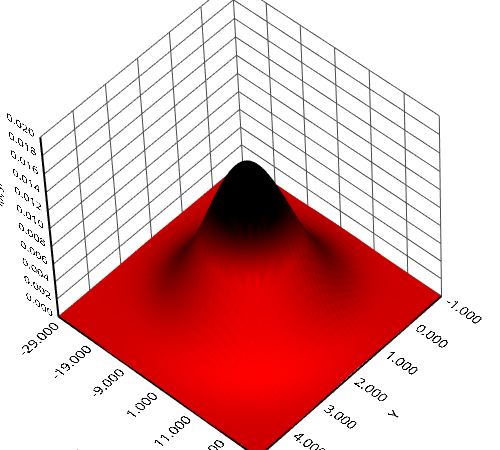
\includegraphics[width=\linewidth]{1.png}
  \caption{ 0 covariance, $\sigma_X > \sigma_Y$}
  \label{fig:boat1}
\end{figure}


\begin{figure}
  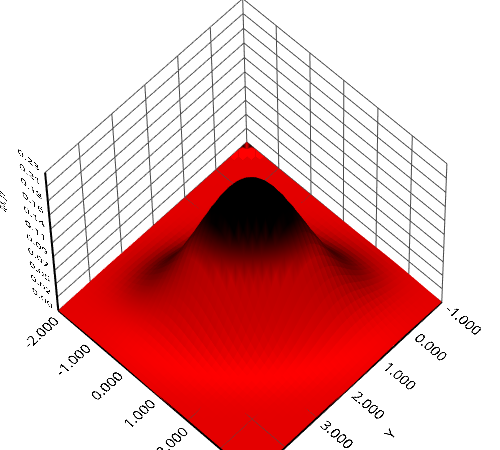
\includegraphics[width=\linewidth]{2.png}
  \caption{ 0.5 covariance, $\sigma_X = \sigma_Y$}
  \label{fig:boat2}
\end{figure}

\section*{Answer 10}
Given $\lambda_{j}=0$, y will be $\lambda_{1}a_{1}+...+\lambda_{j-1}a_{j-1}+\lambda_{j+1}a_{j+1}+...+\lambda_{n}a_{n}$ when we have $a_{1},a_{2}...,a_{j-1},y,a_{j+1},...,a_{n}$ this is basically the same thing as having the set of vectors \{$a_{1},...,a_{n}$\}-\{$a_{j}$\} which by definition can't span/form a basis of $R^{n}$\\\\


\section*{Answer 11}
Say the set \{$v_{1}-v_{2},....,v_{n}$ \}=\{$w_{1},w_{2},...,w_{n}$\}.It is easy to see that we can attain any vector $v_{i}$ through $\sum_{k=i}^{n} w_{k}$. Since we can attain each vector from the original set that spans V using the new set, we can conclude that this new set also spans V.\\\\
	
\section*{Answer 12}
i)We start with det(A-I$\lambda$) =0, \\

$\begin{vmatrix}
 5-\lambda & 4&2\\
 4&5-\lambda &2\\
 2&2&2-\lambda
\end{vmatrix}
$=0 \\
Which gives us $-\lambda^{3}+12\lambda^{2}-21\lambda+10=0$\\
This decomposes into $-(\lambda -1)(\lambda -1)(\lambda -10)=0$\\
For $\lambda_{1,2}=1$ we use the general solution which is:\\
$\begin{bmatrix}
    4&	4& 2\\
    4&	4& 2\\
    2&  2& 1
\end{bmatrix}
$
$\begin{bmatrix}
    x_{1}\\
    x_{2}\\
    x_{3}
\end{bmatrix}
$=$\begin{bmatrix}
    0\\
    0\\
    0
\end{bmatrix}
$ for an eigenvector ($x_{1},x_{2},x_{3}$). From this equality we get $2x_{1}+2x_{2}+x_{3}=0$, if we represent $x_{1}$ in terms of $x_{2}$ and $x_{3}$ the eigenvector takes the form of $\begin{bmatrix}
    \frac{-2x_{2}-x_{3}}{2}\\
    x_{2}\\
    x_{3}
\end{bmatrix}
$ this can be split into two lineary independent vectors :
$x_{2}$
$\begin{bmatrix}
    -1\\
    1\\
    0
\end{bmatrix}
$+$x_{3}$
$\begin{bmatrix}
    \frac{-1}{2}\\
    0\\
    1
\end{bmatrix}
$ which gives our two eigenvectors for the first eigenvalue with multiplicity 2.\\
For $\lambda_{3}=10$ we get two equations namely, $x_{1}-2x_{3}=0$ and $x_{2}-2x_{3}=0$. From these two equations it s easy to deduce that th third eigenvector is $\begin{bmatrix}
    2\\
    2\\
    1
\end{bmatrix}
$.\\
So $\lambda_{1,2}=1$ has eigenvectors $\begin{bmatrix}
    -1\\
    1\\
    0
\end{bmatrix}
$,
$\begin{bmatrix}
    \frac{-1}{2}\\
    0\\
    1
\end{bmatrix}
$ and $\lambda_{3}=10$ has eigenvector$\begin{bmatrix}
    2\\
    2\\
    1
\end{bmatrix}
$\\\\
ii) it is easy to see that the diagnal matrix D in the diagonal form of A=PD$P^{-1}$
equals $\begin{bmatrix}
    1&	0& 0\\
    0&	1& 0\\
    0&  0& 10
\end{bmatrix}
$
and the matrix of eigenvectors P is $\begin{bmatrix}
    -1&	 \frac{-1}{2}& 2\\
    1&	0& 2\\
    0&  1& 1
\end{bmatrix}
$ thus the inverse $P^{-1}$ becomes $\begin{bmatrix}
    \frac{-4}{9}&	 \frac{5}{9}&  \frac{-2}{9}\\\\
     \frac{-2}{9}&	 \frac{-2}{9}&  \frac{8}{9}\\\\
     \frac{2}{9}&   \frac{2}{9}&  \frac{1}{9}
\end{bmatrix} 
$
Thus the diagonal form of A is: $\begin{bmatrix}
    -1&	 \frac{-1}{2}& 2\\
    1&	0& 2\\
    0&  1& 1
\end{bmatrix}
$
$\begin{bmatrix}
    1&	0& 0\\
    0&	1& 0\\
    0&  0& 10
\end{bmatrix}
$
$\begin{bmatrix}
    \frac{-4}{9}&	 \frac{5}{9}&  \frac{-2}{9}\\\\
     \frac{-2}{9}&	 \frac{-2}{9}&  \frac{8}{9}\\\\
     \frac{2}{9}&   \frac{2}{9}&  \frac{1}{9}
\end{bmatrix} 
$\\\\
\section*{Answer 13}
We start by assuming that the condition that all the eigenvalues are positive is non-sufficient and add the condition that the eigenvectors must be orthogonal so that the inverse of the eigenvector matrix must be it's transpose. So $x^{T}Ax$ becomes $x^{T}S\Lambda S^{T}x$ where $\Lambda$ is the diagonal eigenvalue matrix and S is the matrix of eigenvectors. This simplifies into 
$\begin{bmatrix}
    x_{1}&
    \cdots&
    x_{n}
\end{bmatrix}
$
$\Lambda$
$\begin{bmatrix}
    x_{1}\\
    \vdots\\
    x_{n}
\end{bmatrix}
$ where $x_{1},...,x_{n}$ are the results from the vector-matrix multiplication $x^{T}S$ and $xS^{T}$ the only way we can be sure that they are equal to eachother is if the eigenvectors are orthogonal.
Finally when we complete the multiplication we have $x_{1}^{2}\lambda_{1}+...+x_{n}^{2}\lambda_{n}$ from here it is easy to see that this value is positive only if all eigenvalues are positive. So in conclusion not only do all eigenvalues be positive the eigenvectors must be orthognal, which also both happen tobe the properties of positive definite matrices.\\

\section*{Answer 14}
i)Let us say that $x^{T}x$=[$x_{1}^{2}+...+x_{n}^{2}$]=y. So $\nabla_{x}x^{T}x=\nabla_{x}y $ which is $\begin{bmatrix}
    \frac{\partial y}{\partial x_{1}}\\
    \vdots\\
    \frac{\partial y}{\partial x_{n}}
\end{bmatrix}
$=$\begin{bmatrix}
    2 x_{1}\\
    \vdots\\
    2 x_{n}
\end{bmatrix}
$=2x\\\\
ii)Say  $x^{T}Ax$=y, then,y=$\begin{bmatrix}
   x_{1}^{2}a_{11}+x_{1}x_{2}a_{21}+...+x_{1}x_{n}a_{n1}\\
    +\\
    x_{1}x_{2}a_{12}+x_{2}^{2}a_{22}+...+x_{2}x_{n}a_{n2}\\
    +\\
    \vdots\\
    +\\
    x_{1}x_{n}a_{1n}+x_{2}x_{n}a_{2n}+...+x_{n}^{2}a_{nn}
\end{bmatrix}$ \\\\So we have $\nabla_{x}x^{T}Ax=\nabla_{x}y $=$\begin{bmatrix}
    \frac{\partial y}{\partial x_{1}}\\
    \vdots\\
    \frac{\partial y}{\partial x_{n}}
\end{bmatrix}
$=$\begin{bmatrix}
    (2x_{1}a_{11}+x_{2}a_{21}+...+x_{n}a_{n1})+x_{2}a_{12}+x_{3}a_{13}+...+x_{n}a_{1n}\\
    
    x_{1}a_{21}+(x_{1}a_{12}+2x_{2}a_{22}+...+x_{n}a_{n2})+x_{3}a_{23}+...+x_{n}a_{2n}\\
    
    \vdots\\
    
    x_{1}a_{n1}+x_{2}a_{n2}+x_{3}a_{n3}+...+(x_{1}a_{1n}+x_{2}a{2n}+...+2x_{n}a_{nn})
\end{bmatrix}
$\\\\ since A is a symmetric matrix $a_{ij}=a_{ji}$.\\\\ Thus the exression for $\nabla_{x}y$ becomes $\begin{bmatrix}
    2x_{1}a_{11}+2x_{2}a_{12}+...+2x_{n}a_{1n}\\
   
    \vdots\\
    
    2x_{1}a_{n1}+2x_{2}a_{n2}+...+2x_{n}a_{nn}\\
\end{bmatrix}
$=$2Ax$\\\\\\\\\\\\\\
iii)We know that $\nabla_{x}^{2}y$ is just $\nabla_{x}(\nabla_{x}y)$ so using the knowledge we gained from the previous question $\nabla_{x}^{2}x^{T}Ax$=$\nabla_{x}2Ax$ becomes $\nabla_{x}$
$\begin{bmatrix}
    2x_{1}a_{11}+2x_{2}a_{12}+...+2x_{n}a_{1n}\\
   
    \vdots\\
    
    2x_{1}a_{n1}+2x_{2}a_{n2}+...+2x_{n}a_{nn}\\
\end{bmatrix}
$\\\\\\ \indent\indent\indent\indent\indent\indent\indent\indent\indent\indent\indent\indent =\\\\\\$\begin{bmatrix}
    \frac{\partial(2x_{1}a_{11}+2x_{2}a_{12}+...+2x_{n}a_{1n})}{\partial x_{1}}& \cdots &\frac{\partial(2x_{1}a_{n1}+2x_{2}a_{n2}+...+2x_{n}a_{nn})}{\partial x_{n}}\\
   
    \vdots&&\vdots\\
    
    \frac{\partial(2x_{1}a_{n1}+2x_{2}a_{n2}+...+2x_{n}a_{nn})}{\partial x_{1}}&\cdots&\frac{\partial(2x_{1}a_{n1}+2x_{2}a_{n2}+...+2x_{n}a_{nn})}{\partial x_{n}}\\
\end{bmatrix}
$ whcih as you can easily see is just $2A$.
\\\\
\section*{Answer 15}
i)From the Steinitz exchange lemma we know that two sets of bases that form a finite dimensional vector space have the same number of elements\\\\
ii)$A$ is a symmetric matrix with real values which diagonalizes into $S\Lambda S^{-1}$ whixh in this case is $S\Lambda S^{T}$ since S is orthonormal.
Since A is a symmetric matrix it must satisfy $A=A^{T}$. So $(S\Lambda S^{T})^{T}=S^{T^{T}}\Lambda^{T} S^{T}=S\Lambda S^{T}$. Since the conditions are satisfied the statement is true.\\\\
iii)$A$ has diagonal form $S\Lambda S^{-1}$ so $A^{T}$ has diagonal form $S^{T^{-1}}\Lambda S^{T}$. Thus the equality $A^{T}A=AA^{T}$ becomes $S^{T^{-1}}\Lambda S^{T}S\Lambda S^{-1}=S\Lambda S^{-1}S^{T^{-1}}\Lambda S^{T}$ this equality holds only when $S^{-1}=S^{T}$, which only happens when the eigenvectors are orthogonal.\\\\
iv)False in a 3x3 system with repeated eigenvalues we can still obtain linearly independent eigenvectors as we did in the previous questions.\\\\
v)False, consider a matix A=$\begin{bmatrix}
    2&0\\
    0&0
\end{bmatrix}$,p(A)=det(A-I$\lambda$),
$\begin{vmatrix}
    2-\lambda&0\\
    0&-\lambda
\end{vmatrix}$=$\lambda(\lambda-2)$=0,the first eigenvalue is 0.\\\\
vi)True, Since the columns are linearly independent each transformation will be unique.


\section*{Answer 16 - BONUS}



\end{document}


